\documentclass[11pt]{article}

\usepackage{a4wide}
\usepackage{amsmath}
\usepackage{natbib}
\usepackage{booktabs}
\usepackage{graphicx}
\usepackage{tabularx}
%\graphicspath{{expt/}}
\usepackage{times}
\usepackage[varg]{txfonts}
\usepackage{color}
\usepackage{epsfig}
\usepackage{verbatim}
\usepackage[hidelinks]{hyperref}
\usepackage{enumitem}

\parindent=0pt 

\begin{document}

\pagenumbering{arabic}
\title{TN2624 MATLAB Session 11}
\date{May 23, 2013}
%\date{\today}
\maketitle
\begin{quote} 
\begin{enumerate}
\item All practical sessions \textbf{must}
\begin{itemize}
{\color{red}\item be completed between 08:45 AM and 10:30 AM.}
\item be completed in couples (meaning: $n = 2 \pm 0.0$)
\end{itemize}
\item By the end of this practical session you have to submit a MATLAB m-file and a word or pdf file. The MATLAB m-file \textbf{must}
\begin{itemize}
\item be only a single m-file (if you feel the need to define a function in an extra file it can be more than one, of course)
\item contain the code for all questions of this session.
\end{itemize}

\item Both the MATLAB m-file and the word/pdf file \textbf{must}
\begin{itemize}
\item be uploaded by only one of the group members.
\item be named using the {\color{red}NET ID} and {\color{red}STUDENT NUMBER} of the people in your group as follows:\\
	{\color{red}\verb|NETID_NUMBER_NETID_NUMBER_MATLABx.extension|}\\
	or, for those who are working alone:\\
	{\color{red}\verb|NETID_NUMBER_MATLABx.extension|}\\
Here the ‘x’ represents the MATLAB assignment number of the given session and ‘.extension’ will either be ‘.m’ or ‘.doc’/‘.docx’/ ‘.pdf’.\\
E.g.\\
\verb|jhoward_9214200_dschroeder_8438711_MATLAB11.m|\\
\verb|jhoward_9214200_MATLAB11.m|
\end{itemize}

\item The word/pdf file \textbf{must}
\begin{itemize}
\item be written in English.
\item have the answer to each question formatted as follows: 
	\begin{itemize}
	\item MATLAB code if required in the question
	\item answers to all sub-questions, including figures, equations and any other required discussion.
	\end{itemize}
\end{itemize}

{\color{red}
\item Please note:
\begin{itemize}
\item Points will be deducted for missing labels (and legends, if necessary) on plots.
\end{itemize}
}
\end{enumerate}
\end{quote}

\newpage

%%%%%%%%%%%%%%%%%%%%%%%%%%%%%%%%%%%%%%%%%%%%%%%%%%%%%%%%
%%%%%%%%%%%%%%%%%%%%%%%%%%%%%%%%%%%%%%%%%%%%%%%%%%%%%%%%
%%%%%%%%%%%%%%%%%%%%%%%%%%%%%%%%%%%%%%%%%%%%%%%%%%%%%%%%
\noindent\textbf{Constants:}\\

\begin{tabular}{ll}
Boltzmann constant:		&	$k=8.62\cdot10^{-5}\,\mathrm{eVK^{-1}}$\\
Electron mass:			&	$m=5.69\cdot10^{-16}\,\mathrm{eVs^2cm^{-2}}$\\
Planck constant:			&	$h=4.14\cdot10^{-15}\,\mathrm{eVs}$\\
Valence band edge Si		&	$E_\text{V}=0\,\mathrm{eV}$\\
Conduction band edge Si	&	$E_\text{C}=1.12\,\mathrm{eV}$
\end{tabular}\\

(The preferred energy unit in semiconductor physics is the electronvolt (eV), particle densities are given in $\mathrm{cm^{-3}}$. {\bf Use these units in all your calculations and plots.})\\

\section*{Semiconductor statistics Part 1  -- the intrinsic semiconductor (70 pts)}
\label{sec:lot}

\begin{figure}[h]
\centering
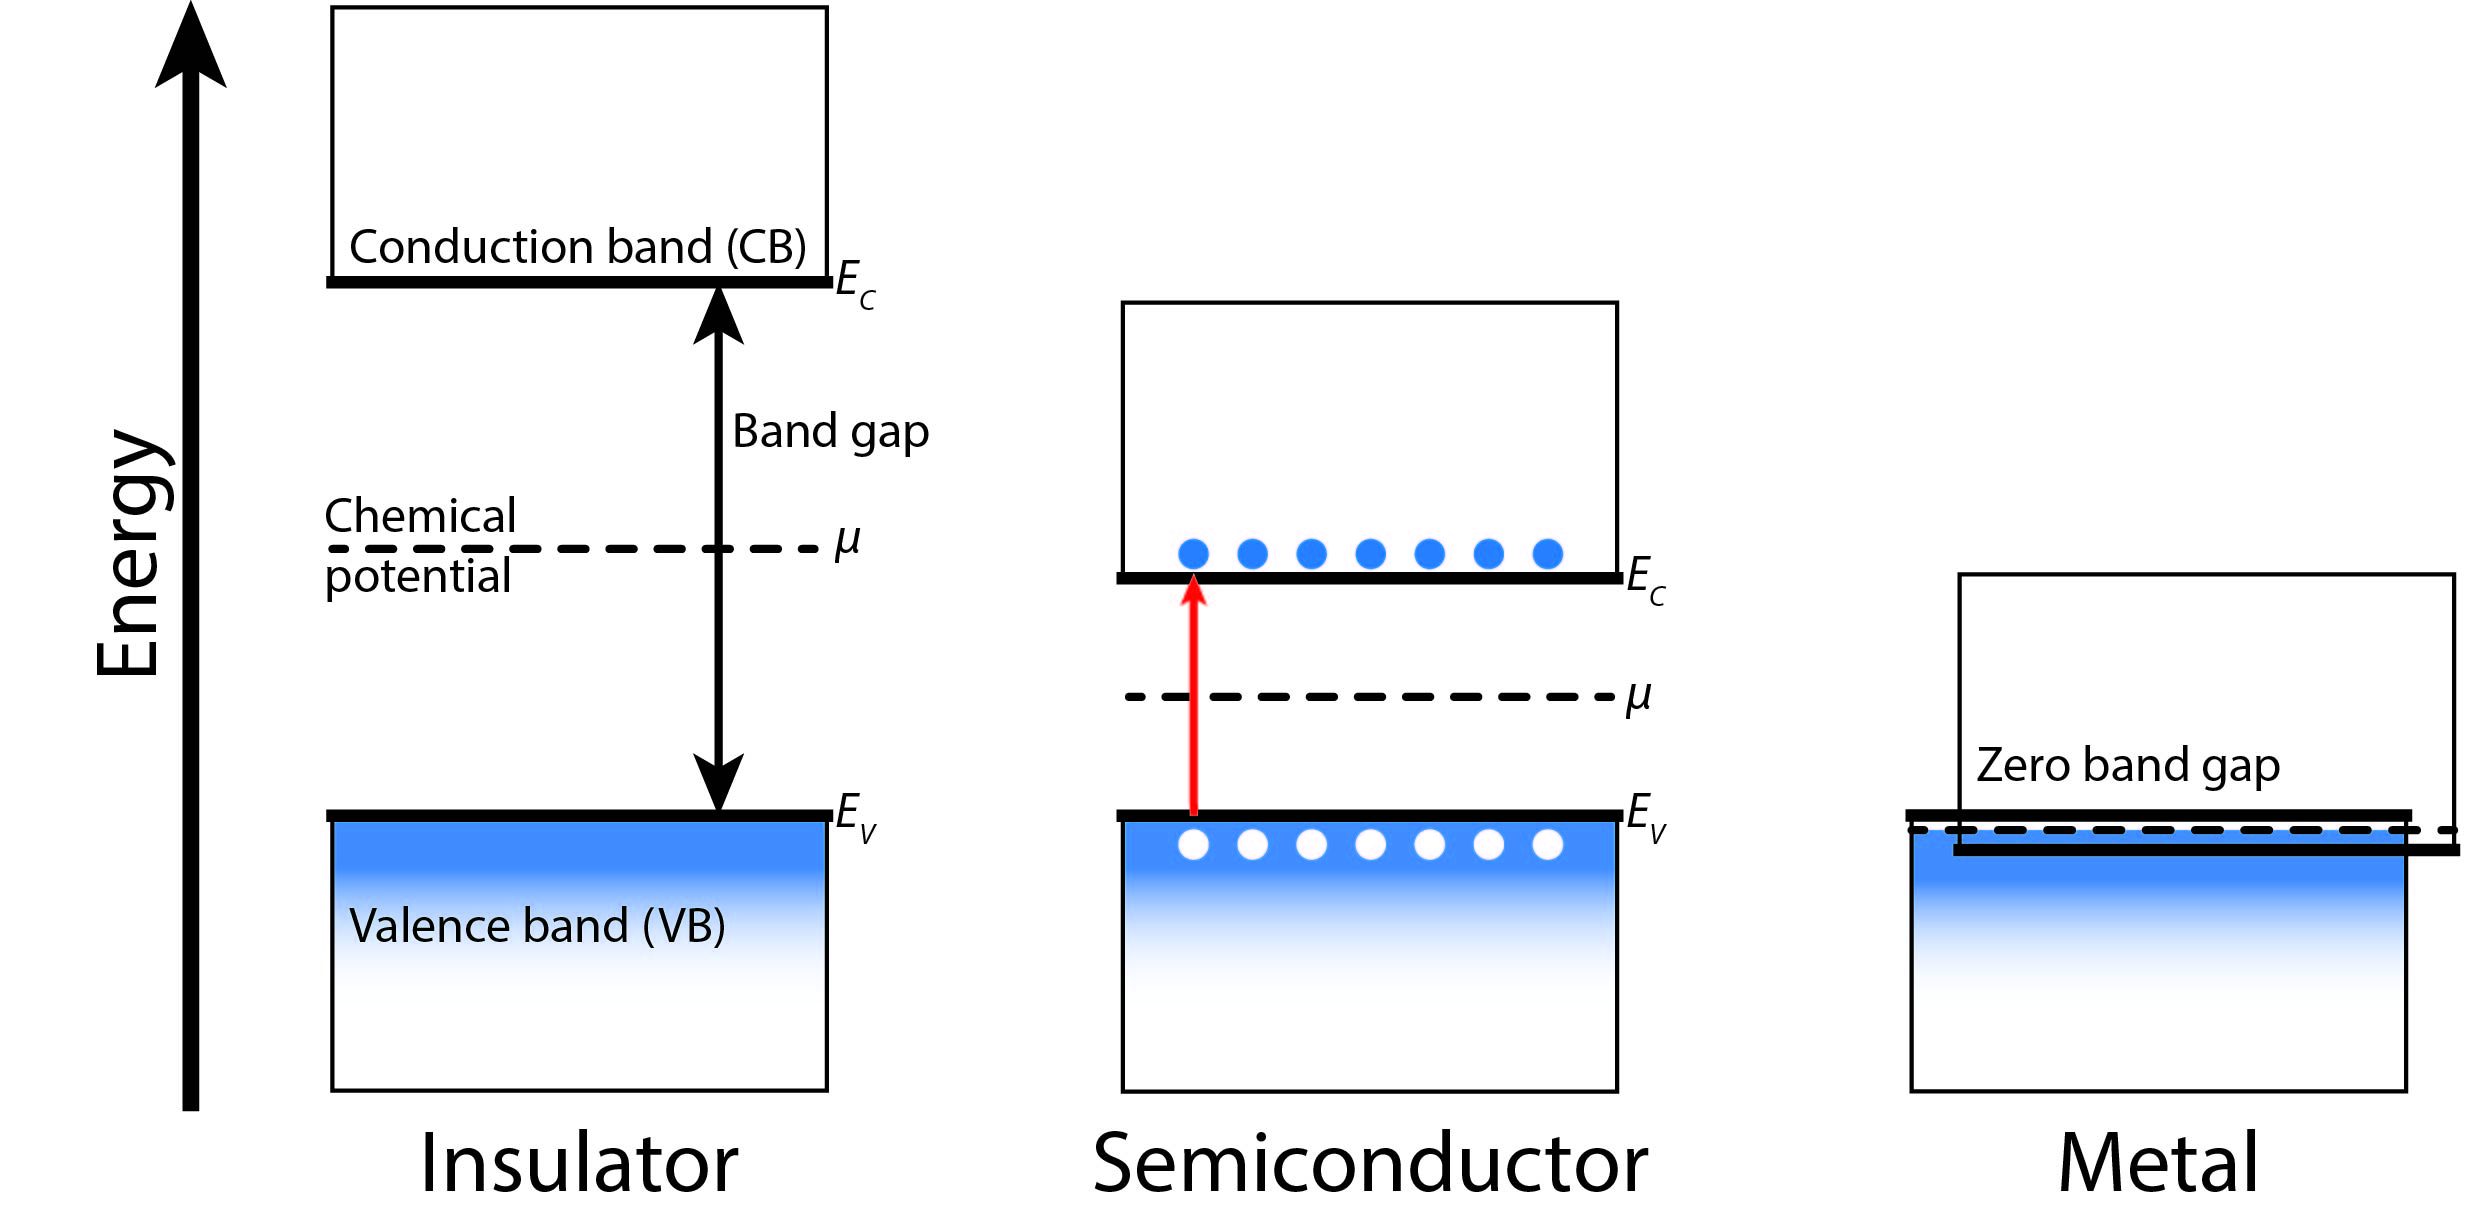
\includegraphics[width=0.8\textwidth]{band_theory.jpg}
\caption{Intrinsic materials}
\label{gaps}
\end{figure}
In solids, the allowed electron energies are no longer given by discrete states. Due to the influence of the large number of ions composing the solids the allowed energies are grouped into bands separated by gaps. The defining property of a \textbf{metal} is the availability of states close to the energy of the chemical potential $\mu$ (see figure \ref{gaps}). In \textbf{insulators} $\mu$ is situated right in the middle of a large gap. This means that at low temperatures the band below the gap is completely filled, while the band above the gap is empty. No current can flow, since the electrons in the lower band have no states close in energy (they are ``stuck''). In a \textbf{semiconductor} the chemical potential is located in the middle of a gap, but the gap is small enough to allow for the thermal excitation of some electrons from the lower band (the {\bf valence band}) to the higher band ({\bf conduction band}) at room temperature. The electron is now missing in the valence band. This ``missing electron'' is called a {\bf hole} and behaves just like an electron with positive charge (this is a rough simplification, but sufficient for our purposes). Take a look at figure (\ref{gaps}). Since the number of electrons in the intrinsic (pure) semiconductor is exactly equal the number of holes, in our simplified model the {\bf chemical potential is located in the middle of the bandgap for all temperatures}. The occupation probability in the conduction band is given by the Fermi-Dirac distribution
$$ \bar {n}_\text{FD,e}(E)=\frac{1}{1+\exp{\frac{E-\mu}{k T}}}.$$ 

For all practical purposes, outside the bandgap the states can be viewed as being {\bf continuously distributed}. For our purposes, all we need to know about these states are the \textbf{densities of state} (states per energy per volume) of the electrons and the holes. In our simplified model they are given by:
\begin{align}
	g_\text{e}(E)&=\frac{\pi(8m)^{3/2}}{2h^3}\sqrt{E-E_\text{C}} \text{ (electrons)}\\
	g_\text{h}(E)&=\frac{\pi(8m)^{3/2}}{2h^3}\sqrt{E_\text{V}-E} \text{ (holes)}
\end{align}
And all we need to know about these densities of state can be summarized as follows:
\begin{itemize}\itemsep0pt
\item $g_\mathrm{e/h}(E)$ times the Fermi-Dirac distribution $\bar {n}_\text{FD,e/h}(E)$ is the {\bf density of electrons/holes per energy per volume} ($\mathrm{eV^{-1}cm^{-3}}$)
\item $n=\int_{E_\text{C}}^\infty g_\text{e}(E) \bar {n}_\text{FD,e}(E) \text{d}E$ and $p=\int_{-\infty}^{E_\text{V}} g_\text{h}(E) \bar {n}_\text{FD,h}(E) \text{d}E$ are the {\bf total densities of electrons and holes, respectively, per volume ($\mathrm{cm^{-3}}$)}.
\end{itemize}
You will learn more about the density of states in next week's lecture.

\begin{enumerate}[resume]
\item\label{item:ex1} \textbf{(25 pts)} Calculate the {\bf Fermi-Dirac distribution of the electrons} $\bar {n}_\text{FD,e}(E)$ as a function of energy. Use \verb|E=-0.5:0.001:1.5| (in eV) for the energy and $T=300\,\mathrm{K}$. Use the constants at the top of this assignment. Assume that the chemical potential is located in the middle of the gap. Then calculate the {\bf densities of states for both holes and electrons} $g_\mathrm{e/h}(E)$ for the same energy range and store them in a single array with two columns. You might want to use the function \verb|real()| to dump the imaginary parts of the roots. Those are of no interest since there are no states in the band gap. Then plot both $\bar {n}_\text{FD}(E)$ and $g_\mathrm{e/h}(E)$ in a single graph. Since the scales of the two functions are very different, you should use \verb|plotyy(E,FD,E,g_eh)| to create a graph with two different y-axes. \verb|FD| is the vector you calculated for the Fermi-Dirac distribution and \verb|g_eh| is the two-dimensional array containing the densities of states for electrons and holes. Use the following code to label the two y-axes and to add some vertical lines at the band edge energies and the chemical potential:
\begin{small}
\begin{verbatim}
[AX,H1,H2] = plotyy(E,FD,E,g_eh)
set(get(AX(1),'Ylabel'),'String','Label Axis 1', ...add the usual style options)
set(get(AX(2),'Ylabel'),'String','Label Axis 2', ...add the usual style options)

yLimit = get(gca,'YLim');
line([EC EC], yLimit, 'color', 'black', 'lineStyle', '-')
line([EV EV], yLimit, 'color', 'black', 'lineStyle', '-')
line([EC/2 EC/2], yLimit, 'color', 'black', 'lineStyle', '--')
\end{verbatim}
\end{small}

{\color{red}In your report: the plot}

\item \label{itm:occhole} \textbf{(5 pts)} What does the {\bf Fermi-Dirac distribution of the holes} look like? Write the {\color{red}equation and a short comment (less than 20 words) in your report}.

\item \label{itm:aa}\textbf{(10 pts)} Calculate the {\bf electron density} (per eV per $\mathrm{cm^3}$) as a function of energy. Do so by multiplying the Fermi-Dirac distribution from exercise \ref{item:ex1} and the corresponding density of states. Plot your result between 1 and $1.5\,\mathrm{eV}$ (\verb|xlim([1,1.5])|). {\color{red}In your report: the plot}

\item \textbf{(5 pts)} Then calculate the {\bf total electron density} (per  $\mathrm{cm^3}$) in intrinsic (pure) silicon at $T=300\,\mathrm{K}$. Use the function \verb|trapz(x,y)| in order to perform the numerical integration of the array obtained in question \ref{itm:aa}. For commercial transistors and diodes charge concentrations are higher than $10^{15}\,\mathrm{cm^{-3}}$. Do you think intrinsic (pure) silicon is a suitable material to build electronic devices? {\color{red}In your report: the value for the electron concentration, a comment on intrinsic silicon}

\item \label{itm:tempdep}\textbf{(25 pts)} Since our intrinsic semiconductor has way too low a {\bf total electron density} (per  $\mathrm{cm^3}$) for most practical applications, we now try to populate the conduction band with more electrons by thermal activation. Define a vector \verb|T=100:100:1500| to explore an extended temperature range. Then calculate the {\bf total electron density} (per  $\mathrm{cm^3}$) just like before, but for each of the temperatures. You can either use meshgrids (\verb|meshgrid(T,E)|) or for-loops (copy and paste your code from above) to calculate the Fermi-Dirac distribution $\bar {n}_\text{FD,e}(E,T)$ and the density of state $g_\text{e}(E,T)$. Get the {\bf total electron density} (per  $\mathrm{cm^3}$) through integration by \verb|trapz()|. Use the function \verb|semilogy()| to {\bf plot the {\bf total electron density} (per  $\mathrm{cm^3}$) semilogarithmically as a function of temperature}. Also add a graph containing {\bf the Fermi-Dirac distribution for the highest and the lowest temperature} (\verb|xlim([-0.1,1.2])|). Add horizontal lines at all relevant energy parameters (band edges, center of band gap). Copy from problem 1.\\
How would you explain the increase of the {\bf total electron density} (per  $\mathrm{cm^3}$) with increasing temperature when looking at those Fermi-Dirac distributions for the two temperatures? Do you think increasing the temperature is a wise approach to adjusting the charge carrier density in the material? {\color{red}In your report: the graph with the {\bf total electron densities} (per  $\mathrm{cm^3}$), the graph with the Fermi-Dirac distributions for different temperatures, short answers to the two questions}

\section*{Semiconductor statistics Part 2 -- the doped semiconductor (30 pts)}
\label{sec:lot}

The more common approach to adjusting the charge carrier concentration in a semiconductor is called {\bf doping}. Each silicon atom in the crystal has {\bf 4} valence electrons. When we introduce atoms with a higher number of valence electrons (called {\bf donors}) into the crystal (e.g. phosphorus, {\bf 5} valence electrons), the additional electron is just loosely bound. It can be {\bf excited easily} to the conduction band, leaving behind a {\bf positively charged ion}. The situation in the energy diagram is shown in figure \ref{donors}. Due to the phosphorus atoms, {\bf additional states} are available {\bf within} the band gap, close to the edge of the conduction band. The energetic distance between the additional states and the conduction band edge is $\Delta E_\text{D}=0.044\,\mathrm{eV}$ in the case of phosphorus atoms in silicon.

\begin{figure}[h]
\centering
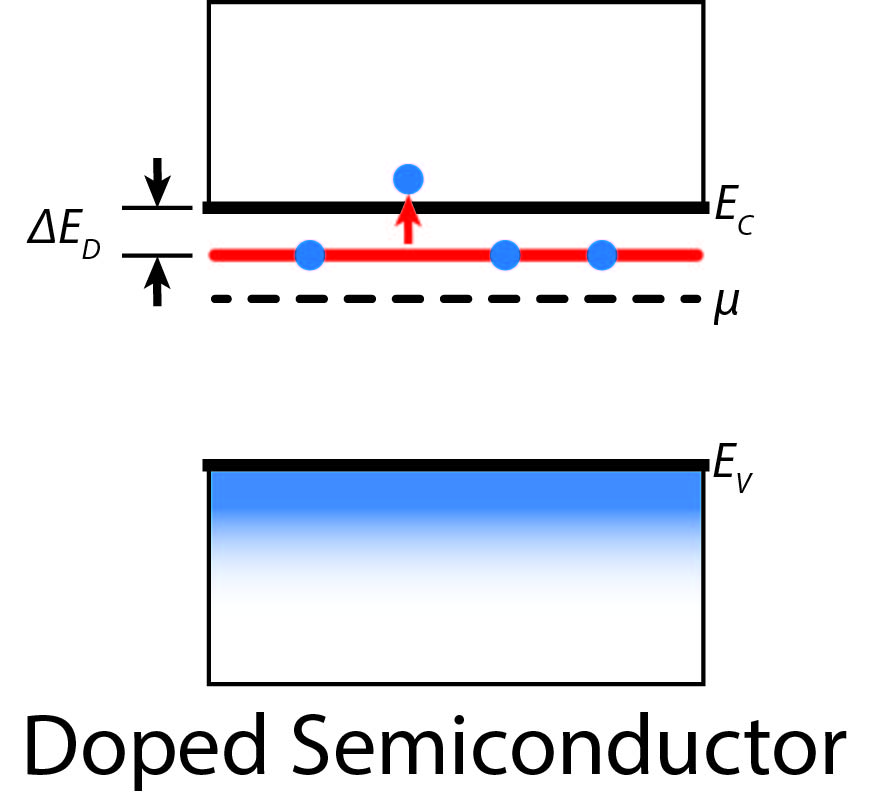
\includegraphics[width=0.3\textwidth]{donorlevels.jpg}
\caption{Donors in semiconductors}
\label{donors}
\end{figure}

If $N_\text{D}$ is the density of donors in the semiconductor host material, the density of {\bf ionized} donors (i.e. the density of electrons in the conduction band stemming from the donors) is given by
\begin{equation}N_\text{D}^+=\frac{N_\text{D}}{1+2\exp\left[-\frac{E_\text{C}-\Delta E_\text{D}-\mu}{kT}\right]}.\label{ion}\end{equation}
(It is a good exercise to derive this equation from the grand partition function. Don't forget that the electron, when bound to the donor atom, can have two independent spin states.)

\item \textbf{(20 pts)} In intrinsic semiconductors, the chemical potential can be assumed to be located in the center of the band gap. This is no longer the case when we introduce donor atoms. One might say that the symmetry between conduction band and valence band is broken (see figure \ref{donors}). Thus, in order to calculate the electron density, we first need to calculate the position of the chemical potential. To do so, we can start from the observation that the total {\bf charge in the semiconductor is conserved in any case}. For every electron in the conduction band there must be either a positive hole in the valence band or a positively ionized donor atom. So:
\begin{equation}\label{chargecons}n(\mu)=p(\mu)+N_\text{D}^+(\mu)\end{equation}
with the total electron density $n(\mu)=\int_{E_\text{C}}^\infty g_\text{e}(E) \bar {n}_\text{FD,e}(E,\mu) \text{d}E$,\\ the total hole density $p(\mu)=\int_{-\infty}^{E_\text{V}} g_\text{h}(E) \bar {n}_\text{FD,h}(E,\mu) \text{d}E$, and $N_\text{D}^+(\mu)$ given by equation (\ref{ion}). This equation {\bf gives us the chemical potential}. All we need to do is to calculate the left-hand side and the right-hand side as a function of the chemical potential, and see for which value of $\mu$ they are equal.\\
Define a vector \verb|mu=0:0.01:1.5| for the chemical potential. Use \verb|T=300| for the temperature and $N_\text{D}=10^{18}\,\mathrm{cm^{-3}}$ for the donor concentration. Calculate the {\bf total electron density} (per  $\mathrm{cm^3}$) as a function of $\mu$. This is equivalent to what you did in problem \ref{itm:tempdep}, just with $\mu$ instead of $T$. Again, use \verb|meshgrid(E,mu)| (easier!) or for-loops. You can copy, paste and adjust your code from the first part of this assignment. Do the same for the holes. Remember that the Fermi-Dirac distribution of the holes is not the same as the one for the electrons (question (\ref{itm:occhole})). $N_\text{D}^+$ is given by equation (\ref{ion}). Plot the left-hand side and the right-hand side of equation (\ref{chargecons}) in a {\bf single semilogarithmic graph}: \verb|semilogy(mu,p.'+NDp, mu,n)|. Find the value of $\mu$ where they cross (the minimum of the absolute values of their difference). To what {\bf total electron concentration} does this correspond? What's the {\bf total concentration of the holes} in this case?  {\color{red}In your report: one plot, the value of $\mu$, two concentrations}

\item \textbf{(10 pts)} Now we want to know what happens to the {\bf total electron density} (per  $\mathrm{cm^3}$) in a doped semiconductor if we change the temperature over a wide range: \verb|T=50:50:1000|. Use $N_\text{D}=10^{16}\,\mathrm{cm^{-3}}$ and \verb|mu=0:0.001:EC| (a high resolution in energy is critical to obtain accurate results). Just copy the rest of the code from the last question to a for-loop to calculate the total electron density $n(T)$ for the different temperatures. Plot $n(T)$ {\bf semilogarithmically as a function of $1/T$}: \verb|semilogy(1./T,n,'o-')|. Three regions with qualitatively different behavior can be observed. What's going on in each of them? Explain. Then plot the chemical potential as a function of the temperature. Add horizontal lines at all relevant energy parameters (band edges, center of band gap, donor state energy). E.g.:
\begin{verbatim}
xLimit = get(gca,'XLim');
line(xLimit,[EC EC], 'color', 'r', 'lineStyle', '-')
\end{verbatim}
{\color{red}In your report: two plots, the interpretation of the three regions}

\end{enumerate}

\end{document}